
\section{Extracción de noticias desde la web de un municipio}


La extracción de información es uno de los puntos clave del proyecto. Extraemos información de varias fuentes, siendo la más importante de ellas la web oficial del ayuntamiento de cada municipio. El caso que vamos a estudiar es el de aquellos ayuntamientos que hacen uso del gestor de contenidos OpenCMS, ya que se puede suponer que la estructura de las páginas serán similares al estar creadas con la misma herramienta. 

Tras un estudio inicial para determinar la estructura interna de estas páginas hemos determinado siete formas distintas de estructurar los contenidos de la web. Como tenemos varios grupos, el primer paso es determinar a partir de la dirección web la ruta hacia las noticias, una vez queda determinada la ruta se procede a la extracción de las noticias. Para cada grupo se ha creado un script en Python para extraer las noticias según su estructura. Por último se trata la información obtenida para adecuarla nuestra base de datos.

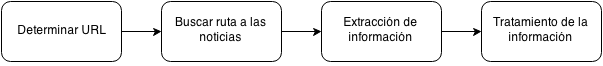
\includegraphics[width=\textwidth]{Extraccion/imagenes/extraccion.png} 

\subsection{Obtención de ruta hacia la información}

Las páginas que hacen uso del gestor de contenido OpenCMS no almacenan la página principal en el directorio raíz del servidor, en la mayoría de casos esta se encuentra bajo la ruta  \textit{.../opencms/opencms/X} donde \textit{X} es normalmente el nombre del municipio, por ejemplo, para Andújar la página del municipio es http://andujar.es/ y la ruta que genera OpenCMS es http://andujar.es/opencms/opencms/andujar/. El determinar esta parte de la ruta a veces es un proceso simple pues al hacer una petición HTTP al servidor la URL de respuesta ya es la ruta completa por lo que hay una redirección automática y solo hay que seguirla.

Cuando no se da la redirección automática el servidor devuelve un pequeño código HTML en el que utiliza el atributo \textit{HTTP-EQUIV} para forzar al navegador a hacer un refresco de la página con la dirección completa, en este caso hacemos, de nuevo, uso de expresiones regulares para obtener la parte extra que añade OpenCMS y construir la dirección completa que nos lleva a la página principal del ayuntamiento que estamos estudiando.

También puede ocurrir que no se dé la redirección automática y que no se devuelva el código anterior sino que directamente se muestra la página principal sin que se vea ningún cambio en la URL, en este caso lo que se hace es buscar todos los enlaces internos de la página principal haciendo uso de expresiones regulares, ya que incluyen la parte de OpenCMS que buscamos, y partimos los enlaces en tantas partes como caracteres ''/'' tenga el enlace y nos quedamos con las tres primeras partes para reconstruir parcialmente el enlace, estos enlaces parciales se guardan en una lista para que una vez tenemos todos enlaces poder buscar el elemento más común de la lista, que será la parte de la dirección que nos falta.

Una vez que tenemos la ruta completa, hacemos un repaso por los enlaces internos para determinar la estructura de la página y se compara con los siete grupos que obtuvimos en el análisis inicial intentando acceder a distintas rutas conocidas probando cuál de ellas es correcta y no devuelve ningún código de error al hacer la petición HTTP para obtener la ruta hasta la información que deseemos buscar, en este caso las noticias. Cuando se tiene la ruta a la información que se desea extraer se lanza el script correspondiente para comenzar a extraer información.

\subsection{Extracción de noticias}

Una vez tenemos la ruta hacia las noticias hay dos casos bien diferenciados, el primero es que las noticias se encuentren ordenadas por categorías, o por el contrario las noticias se encuentran todas en el mismo lugar sin ningún tipo de organización.

Si ya se encuentran ordenadas por categorías las almacenamos en nuestra base de datos respetando la categoría que se le da en la web. 

Si en la web no se le asigna una categoría, las guardamos bajo una categoría especial para posteriormente, durante la fase de tratamiento de la información, asignarles una categoría de un conjunto creado por nosotros mismos. 

Los atributos que almacenamos de cada noticia, además de una categoría, son: Fecha, Municipio, Titular, Resumen, Cuerpo y la URL a la noticia.

En ambos casos el proceso que se sigue para extraer las noticias es común, lo primero es acceder al código HTML donde se encuentra la información, para ello hacemos uso de la librería urllib2 para hacer la petición HTTP y guardar la respuesta, que si no se ha habido ningún problema será el código HTML. Una vez tenemos el código completo hacemos uso de la librería BeutifulSoup, uno de los parseadores de HTML para Python más utilizados actualmente. 
\begin{lstlisting}
cat = Categoria.objects.filter(etiqueta__exact = "sin_categoria")
try:
	respuesta = urllib2.urlopen(url)
except:
	return []
soup = BeautifulSoup(respuesta)
noticias = soup.body.find_all('div', attrs={'class' : 'result group'})	
for element in noticias:
	fecha = None
	titular = None
	enlace = None
	cuerpo = None
	fecha = element.text
	fecha = re.findall("\[(.*?)\]", fecha)
	if len(fecha) != 0:
		fecha = fecha[0]
		fecha = fecha.split("/")
		dia = date(day = int(fecha[0]), month = int(fecha[1]), year = int(fecha[2]))
	else:
		dia = None
	titu = element.find('a')
	if titu is not None:
		titular = titu.text
		titular = modifica_string.elimina_blancos(titular)
		titular = modifica_string.elimina_char_especial(titular)
		titular = titular.replace("\n", "-")
		partes = url.split('/')
		U = partes[0]+'//'+partes[2]
		enlace = U + titu.get('href')
	cuerpo = element.find('span')
	.
	.
	.	.
\end{lstlisting}
Con esta librería seleccionamos y extraemos el contenido de las etiquetas HTML que contienen la información que buscamos, a veces  sacamos dicha información haciendo uso de expresiones regulares y otras simplemente guardamos el texto que queda dentro de las etiquetas. Como obtenemos el enlace a la noticia completa también accedemos a esta dirección para obtener el texto completo de la noticia y en algunos casos la fecha si no ha sido posible obtenerla en el paso anterior. Una vez se ha extraído toda la información posible se construye el enlace a la siguiente página de noticias y seguir extrayendo información de manera recursiva. Como condición de parada de la recursividad tenemos la ocurrencia de algún error en la petición HTML, como un error 404, o que en el código se indique que ya no es existen más páginas para seguir trabajando. 

Una vez se han extraído todas las noticias de un municipio, o de una categoría dentro de un municipio se almacenan en la base de datos ordenadas por orden de publicación, siendo la última la más recientemente publicada.

\subsection{Almacenamiento de la información}

A la hora de almacenar la información obtenida en concreto los resúmenes y los textos completos de las noticias nos hemos encontrado con determinados caracteres que no son admitidos por el gestor de base de datos. El origen de estos caracteres especiales está en que posiblemente OpenCMS ofrezca formularios para permitir al usuario publicar información y en ese formulario se copie el texto de otros programas que si admiten estos caracteres especiales como editores de texto, por lo que el primer paso es eliminar dichos caracteres, para ello repasamos todo el texto eliminando caracteres que queden fuera de la codificación UTF-8. 

Otra situación que nos obliga a hacer tratamiento del texto obtenido son los fallos que contiene el código de las propias páginas web, ya que en muchos casos las etiquetas no están correctamente cerradas lo que hace que parte del código y comentarios se interpreten como texto por la librería BeautifulSoup. Estos fallos en ocasiones provocan una visualización incorrecta de la web.

En este apartado la tarea principal es realizar la clasificación automática de aquellas noticias que se encuentren sin clasificar. Para ello buscamos aquellas palabras que tienen relevancia en cada categoría para poder comparar el texto de cada noticia con estos conjuntos de palabras y determinar con la mayor certeza posible a que categoría pertenece.



\subsection{Sistema tolerante a fallos}

Como dependemos de Internet para realizar esta tarea, es posible que se produzcan fallos en la conexión. Para poder recuperar la tarea de extracción sin tener de iterar de nuevo por todos los pueblos, se ha creado un sistema tolerante a fallos. Cada vez que se termina de buscar nuevas noticias en un municipio se almacena un estado que indica que el proceso ha terminado correctamente. En el caso de error, en la base de datos queda un estado que indica que el proceso no se ha completado.

Para recuperarse en caso de error se vuelve a lanzar el proceso de búsqueda de noticias que buscará posibles errores en la base de datos para realizar la búsqueda solo con aquellos pueblos que sean necesarios.

\subsection{Resultados de la extracción}

Tras realizar la fase de extracción de noticias y buscar noticias nuevas de forma posterior, contamos con 59177 noticias de 95 pueblos distintos, la distribución de los datos es la siguiente:
\begin{center}
\begin{figure}[h]
\centering
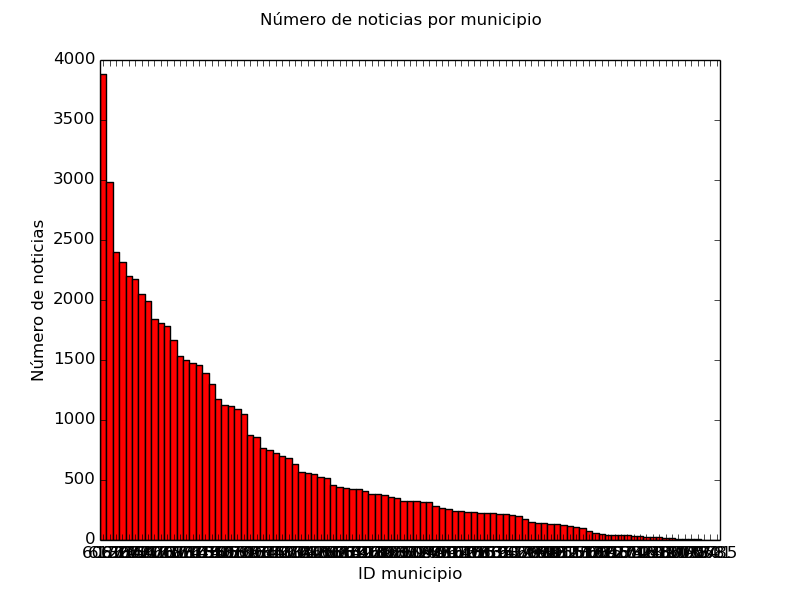
\includegraphics[scale=0.6]{Extraccion/imagenes/histograma.png}
\caption{Número de noticias por municipio}
\end{figure}
\end{center}
Los pueblos con más noticias son:
\begin{center}

\begin{multicols}{2}
\begin{enumerate}
\item Castilblanco de los Arroyos %(3828 noticias)
\item Mairena del Alcor %(2927 noticias)
\item Benalup-Casas Viejas %(2354 noticias)
\item Pedrera %(2293 noticias)
\item Punta Umbría %(2167 noticias)
\item Tocina %(2122 noticias)
\end{enumerate}
\end{multicols}
\end{center}

A continuación se muestra la figura \ref{fig:noti_provincia} donde se muestra en número de noticias ordenado por provincias y la figura \ref{fig:noti_year} muestra el número de noticias por año de publicación.
\begin{center}
\begin{figure}[h]
\centering
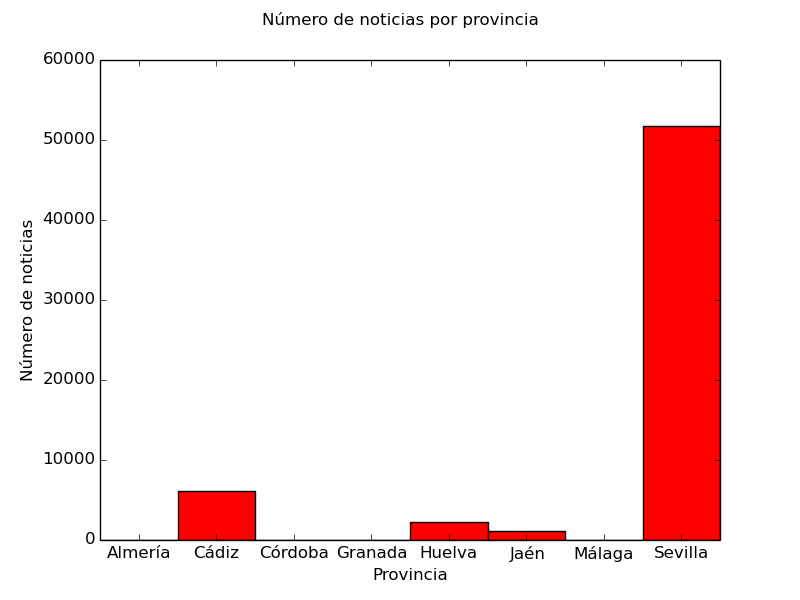
\includegraphics[scale=0.65]{Extraccion/imagenes/histograma_provincias.png}
\caption{Número de noticias por provincia}
\label{fig:noti_provincia}
\end{figure}
\end{center}
%
%
%
\begin{center}
\begin{figure}[h]
\centering
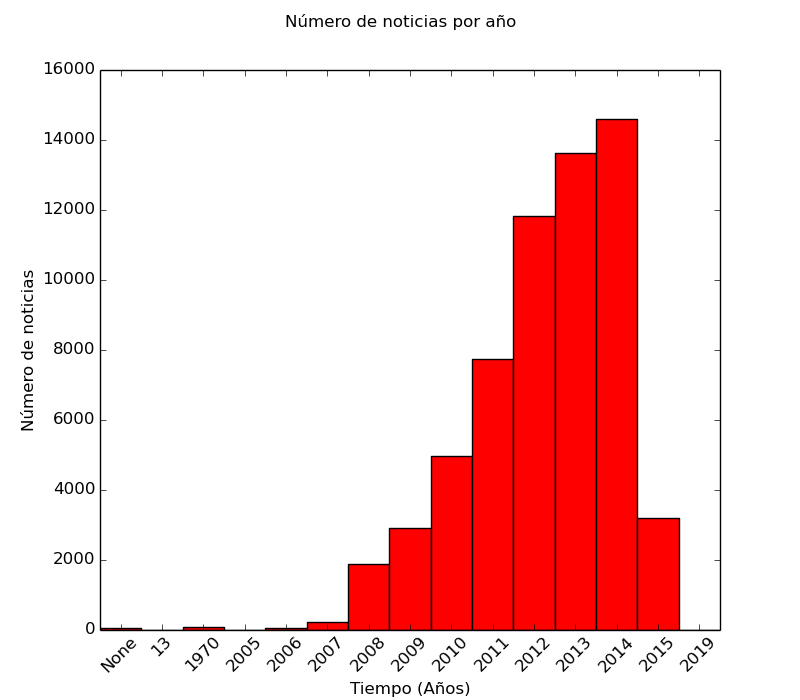
\includegraphics[scale=0.6]{Extraccion/imagenes/histograma_year.png}
\caption{Número de noticias por año}
\label{fig:noti_year}
\end{figure}
\end{center}
%\newpage

\begin{center}


\begin{table}[h]
\begin{tabular}{ll}
\multicolumn{2}{l}{Tras la fase de extracción, disponemos de la siguiente información:}                \\
\textbf{Nombre:}                     & Punta Umbría                                                                                    \\
\textbf{Provincia:}                  & Huelva                                                                                          \\
\textbf{Código:}                     & 21060                                                                                           \\
\textbf{Latitud:}                    & 37.1852585                                                                                      \\
\textbf{Longitud:}                   & -6.9704976                                                                                      \\
\textbf{URL:}                        & http://www.ayto-puntaumbria.es/                                                                 \\
\textbf{Deuda:}                      & 1140 Euros                                                                                      \\
\textbf{Habitantes:}                 & 14976 habitantes                                                                                           \\
\textbf{Superficie:}                 & 38.77 $Km^{2}$                                                                                        \\
\textbf{Densidad población:}         & 386.28 $habitantes/Km^{2}$                                                                            \\
\textbf{Página Wikipedia:}           & http://es.wikipedia.org/wiki/Punta\_Umbría                                                      \\
\textbf{Contratos indefinidos 2013:} & 300                                                                                             \\
\textbf{Contratos temporales 2013:}  & 9489                                                                                            \\
\textbf{Noticia:}                    & Punta Umbría comienza mañana martes sus actos... \\
\textbf{Noticia:}                    & Punta Umbría rotula hoy y mañana vías con el nombre...                        
\end{tabular}
\end{table}
\end{center}